
\documentclass[10pt]{article}

\usepackage{graphicx,amsmath,amssymb,subfigure,enumerate,versions}
\usepackage{multicol,multirow,mdframed}
\usepackage{epstopdf}
\usepackage{pstricks,auto-pst-pdf}
\usepackage{pst-all}
\usepackage{pst-ode}
\usepackage{pst-math}
\DeclareGraphicsExtensions{.png,.jpg,.pdf}

% ************ Page Margins *************
\hoffset=-1.3in
\setlength{\textwidth}{7.5in}
%%%%% MARGINS
\topmargin 0pt
\advance \topmargin by -\headheight
\advance \topmargin by -\headsep
\textheight 9.5in

% ************ Shortcuts *************
\newcommand{\Z}{\mbox{\sf Z\hspace{-1.5mm}Z}}
\newcommand{\SolutionSeparator}{ \hfill \hfill \hrule \hfill \hfill }
\newcommand{\R}{\mbox{\rm I\hspace{-0.75mm}R}}
\columnsep=0.75in
\newcommand{\vsc}{\vspace{1mm}}
\newcommand{\D}{\Delta }
\newcommand{\ifd}{f(x)~dx}
\newcommand{\dd}{\frac{dy}{dx} \,} 
\newcommand{\der}[2]{\frac{d{#1}}{d{#2}} \,}
\newcommand{\ddx}[1]{\frac{d {#1}}{dx} \,} 
\newcommand{\ddy}[1]{\frac{d {#1}}{dy} \,} 
\newcommand{\ddz}[1]{\frac{d {#1}}{dz} \,} 
\newcommand{\ddt}[1]{\frac{d {#1}}{dt} \,} 
\newcommand{\ds}{\displaystyle } 
\newcommand{\la}{\lambda } 
\newcommand{\del}{\nabla } 
\newcommand{\zx}{\frac{\partial z}{\partial x} \,}
\newcommand{\zy}{\frac{\partial z}{\partial y} \,}
\newcommand{\dx}{\frac{\partial f}{\partial x} \,}
\newcommand{\dy}{\frac{\partial f}{\partial y} \,}
\newcommand{\pp}[2]{\frac{\partial {#1}}{\partial {#2}} \,}
\newcommand{\ppx}{\frac{\partial }{\partial x} \,}
\newcommand{\ppy}{\frac{\partial }{\partial y} \,}
\renewcommand{\thesection}{\Roman{section}}
\newcommand{\vi}{\vec{i}}
\newcommand{\vj}{\vec{j}}
\newcommand{\vk}{\vec{k}}
\newcommand{\vv}{\vec{v}}
\newcommand{\lan}{\left\langle}
\newcommand{\ran}{\right\rangle}
\newcommand{\degr}{^{\circ}}

% *** Define the printed question style ***
\newcommand{\q}[1]{ {\em #1} }
% \renewcommand{\q}[1]{ {} }

\newcommand{\notice}{ \begin{center}Some problems and solutions
    selected or adapted from \\ Stewart {\em Calculus-Early
      Transcendentals} and Hughes-Hallett {\em Calculus} .\end{center}
}

% *** Overwrite, if desired, the question format
\input{DocumentFormat.tex}

% *** Footnoting with symbols ***
\long\def\symbolfootnote[#1]#2{\begingroup%
\def\thefootnote{\fnsymbol{footnote}}\footnote[#1]{#2}\endgroup}

\newcommand{\WeekTitleOne}{Derivatives - Foundations}
\newcommand{\WeekTitleTwo}{Derivatives - Linearization and Applications}
\newcommand{\WeekTitleThree}{Derivatives - Applications}
\newcommand{\WeekTitleFour}{Integrals - Foundations}
\newcommand{\WeekTitleFive}{Integrals - Techniques}
\newcommand{\WeekTitleSix}{Integrals - Modeling}
\newcommand{\WeekTitleSeven}{Differential Equations - }
\newcommand{\WeekTitleEight}{Differential Equations - }
\newcommand{\WeekTitleNine}{Differential Equations - }
\newcommand{\WeekTitleTen}{Linear Algebra - }
\newcommand{\WeekTitleEleven}{Linear Algebra - }
\newcommand{\WeekTitleTwelve}{Linear Algebra - }


\usepackage{bbding} % for Checkmarkbold
\begin{document}

\newcommand{\ub}{\underbrace}

\begin{center}
\subsection*{MNTC P01 - Week \#6 - \WeekTitleSix}
\end{center}

\subsection*{Numerical Integration}

\begin{Question} As part of this assignment, you should be able to reproduce the
  LHR rule calculations in MATLAB using a loop. You should know how to
  adapt it to handle either data from a file, or a function defined by
  a formula, as the case requires.
\end{Question}

\begin{enumerate}[1.]
% ******************************
\item \begin{Question}
{\bf Theory} Consider the problem of estimating the general form
  of the integral $$\int_a^b f(x)~dx$$
\begin{enumerate}[(a)]
\item Assume $f(x)$ is a smooth and continuous function.  For our the
  Left-Hand sum, LEFT($n$), by what factor do we reduce the error if
  we use 10 times the number of intervals?

\item Evaluate the integral $\ds \int_0^6 \cos(x)~dx$ exactly, using
  anti-derivatives and the Fundamental Theorem of Calculus.

\item Confirm your answers to part (a) by finding the change in the
  error for LEFT($n$) for the same integral, $\ds \int_0^6 \cos(x)~dx$
  using $n=20$, $n=200$, and $n = 2000$.  Find the error with each $n$
  value, and then compute the ratio of the errors each time you use 10$\times$ as many intervals.
\end{enumerate}
\end{Question}

\begin{Solution}
\begin{enumerate}[(a)]
\item If $f(x)$ is a smooth function, if we use 10 times the
  intervals, the error for LHR's estimate will drop by a factor of $\frac{1}{10}$
\item We can evaluate the integral based on our earlier study of
  derivatives. The only thing to be careful of is that the input
  values will be in radians (not degrees).
  \begin{align*}
    \int_0^6 \cos(x)~dx = \sin(x) \Big|_0^6 = \sin(6) - \sin(0) = -0.279415498
  \end{align*}

\item  The linked script below computes LEFT($n$) for $n=20, 200$ and 2000.  It also computes
the error for each of those integral estimates. 

\href{http://www.mast.queensu.ca/~apsc171/MNTCP01/PracticeProblems/MATLAB/W06CosineIntegral.m}{W06CosineIntegral.m}

Here are the results from the script (with the values for \verb@I@
being the integrals, and \verb@Err@ being the error in the estimates.

\lstinputlisting[showstringspaces=false]{MATLAB/W06CosineIntegral_results.txt}

\end{enumerate}

We can see that as we increase the number of intervals by a factor of
10, the error in the LEFT($n$) estimate is scaled by a factor of
(approximately) $\ds \frac{1}{10}$.

\begin{itemize}
\item When going to $n=200$ from $n=20$, the error ratio is $\ds \frac{6.184021769584658e-04}{0.008073223414391} \approx 0.07 \approx 0.1$ or $\ds \frac{1}{10}$.
\item When going to $n=2000$ from $n=200$, the error ratio is $\ds \frac{5.995413167569907e-05}{6.184021769584658e-04}
 \approx 0.097\approx 0.1$ or $\ds \frac{1}{10}$.
\end{itemize}


\end{Solution}

% ******************************
\item \begin{Question}
For each of the following integrals, 
\begin{itemize}
\item Evaluate the integral exactly, 
\item use MATLAB to compute the LEFT(1000) integral estimate, and
\item comment on the agreement between the results.
\end{itemize}
\begin{enumerate}[(a)]
\item $\displaystyle \int_0^5 x^3 - 5~dx$  
\item $\displaystyle \int_1^{10} \log_{10}(x)~dx$ 
\item $\displaystyle \int_{-1}^{1} x^2 e^{x^3}~dx$ 
\end{enumerate} 
  \end{Question}

\begin{Solution}
 \begin{enumerate}[(a)]
\item Exact value: $\displaystyle \int_0^5 x^3 - 5~dx = \frac{x^4}{4} - 5x \Big|_0^5 = 
\left(\frac{5^4}{4} - 5(5)\right) - (0-0) = 131.25$ \\
LEFT(1000) estimate (see link below to the script that computed this):  130.9377

The agreement is pretty good, with the LEFT(1000) within 1\% of the exact value.

\item $\displaystyle \int_1^{10} \log_{10}(x)~dx $.\\ This requires
  integration by parts, and remembering the derivative rule for
  non-base-$e$ logarithms:
  $\ds \frac{d}{dx} \log_{10}(x) = \frac{1}{x \ln(10)}$ Computing the
  integral (without the $x=1$ and $x=10$ for now to keep the notation
  simpler):
    \begin{align*}
\mbox{ We choose }       u & = \log_{10} x&\mbox{ and } dv & = dx \\
\mbox{ so } du & = \frac{1}{x \ln(10)} ~dx& \mbox{ and } v & = x 
    \end{align*}
Using the integration by parts formula, 
\begin{align*}
  \int \log_{10} x~dx & = x (\log_{10} x) 
- \int x \frac{1}{x \ln(10)}~ dx \\
& = x \log_{10} x - \int \frac{1}{\ln(10)} ~dx \\
& = x \log_{10} x - \frac{x}{\ln(10)} + C  
\end{align*}
This gives the definite integral value of 
\begin{align*}
\int_1^{10} \log_{10}(x)~dx  & = \left(x \log_{10} x - \frac{x}{\ln(10)} \right) \Big|_1^{10} \\
& = \left(10 \log_{10}(10) - \frac{10}{\ln(10)}\right) 
- \left(1 \log_{10}(1) - \frac{1}{\ln(10)}\right)  \\
&  = 10 - \frac{10}{\ln(10)} + \frac{1}{\ln(10)} \\
& \approx 6.0914
\end{align*}
LEFT(1000) estimate (see link below to the script that computed this):  6.0868

The agreement is better for this function, with the LEFT(1000) within 0.1\% of the exact value.

\item $\displaystyle \int_{-1}^{1} x^2 e^{x^3}~dx$ 

This integral can be evaluated exactly using a substitution.

  \begin{align*}
    \mbox{Let }w & = x^3, \mbox{ so } dw=3x^2~dx \mbox{ or } dx = \frac{1}{3x^2}~dw\\
    \int x^2 e^{x^3}~dx & = \int x^2 e^w \left(\frac{1}{3x^2}~dw\right) = \int \frac{1}{3} e^w dw = \frac{1}{3} e^w + C = \frac{1}{3} e^{x^3} + C \\
\end{align*}
This gives the definite integral value of
\begin{align*}
\int_{-1}^{1} x^2 e^{x^3}~dx  & = \frac{1}{3} e^{x^3} \Big|_{-1}^1 \\ 
& = \frac{1}{3}\left( e^1 - e^{-1}\right) \\
& \approx 0.7834 
\end{align*}
LEFT(1000) estimate (see link below to the script that computed this):  0.7811

The agreement is good for this function, with the LEFT(1000) within 1\% of the exact value.
\end{enumerate} 
Link to the MATLAB code: \\
\href{http://www.mast.queensu.ca/~apsc171/MNTCP01/PracticeProblems/MATLAB/W06LeftExamples.m}{W06LeftExamples.m}
\end{Solution}


% ******************************
\item 
  \begin{Question}
    Use the \verb#integral# function to estimate the following
    integrals, and print the estimates with at least 8 digits after
    the decimal.  Use the default accuracy for the \verb#integral#
    function.  Note that the exact values for these integrals were
    computed in the previous question, so we can compare the
    \verb@integral@ estimate to the exact values.
\begin{enumerate}[(a)]
\item $\displaystyle \int_0^5 x^3 - 5~dx$  (exact value: $\displaystyle \frac{5^4}{4} - 25$)
\item $\displaystyle \int_1^{10} 4 \log_{10}(x)~dx$ (exact value: 
$\displaystyle \frac{(-36+40 \ln(2)+40 \ln(5))}{\ln(2)+\ln(5)}$
\item $\displaystyle \int_{-1}^{1} x^2 e^{x^3}~dx$ 
\end{enumerate}
  \end{Question}

\begin{Solution} 
Code that does this would be e.g.
\begin{verbatim}
clc
format long
f = @(x) x.^3 - 5;
a = 0;
b = 5;
I = integral(f, a, b);
exact_value = (5^4/4 - 5*5);
[exact_value, I]  % display both the exact value and the integral estimate
\end{verbatim}
A link to the full MATLAB script for all the examples is included below.

The results are
\begin{enumerate}
\item function: \verb#f = @(x) x.^3 - 5;# \\
estimated integral: 131.25000000
\item function: \verb#f = @(x) log10(x);# \\
estimated integral: 6.091349662870734
\item function: \verb#f = @(x) x.^2 .* exp(x.^3);#\\
estimate integral: 0.783467462429201
\end{enumerate}
Note that all these values are the same as the exact values for all or
almost all the digits shown (12 digits of accuracy).  This is a lot
better performance than using the LEFT($n$) approach, and is actually
easier to code because the \verb@integral@ function is built into
MATLAB.

Link to the MATLAB code: \\
\href{http://www.mast.queensu.ca/~apsc171/MNTCP01/PracticeProblems/MATLAB/W06IntegralExamples.m}{W06IntegralExamples.m}
\end{Solution}

% ******************************
\item 
  \begin{Question}
    The width (in feet) of the golf course fairway was measured at
    100-foot intervals as indicated on the figure.  Estimate the square
    footage of of the fairway.  
    
    \begin{center}
      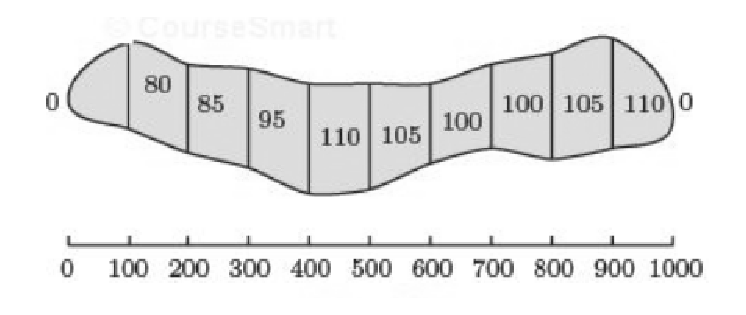
\includegraphics[width=0.5\linewidth]{graphics/Week06_IntegrationApplications/GolfHole}
    \end{center}
  \end{Question}
  
  
\begin{Solution}
  {\bf NOTE: } In this problem, because we are only given data and not
  a function, the only technique we have that would work is LEFT($n$).
  We {\bf can't} use the Fundamental Theorem or the \verb@integral@
  function because both of those require a formula for the function
  that we don't have.

The key steps are:
\begin{enumerate}[1.]
\item Create a vector of the widths, {\em including} the zero widths
  at the start and end of the fairway.
\item Note that  $\Delta x$ = 100 feet for each left-to-right distance.
\item Note that there are 10 intervals (11 widths), so we will be performing a LEFT(10) calculation.
\item Approximate the area on each left-to-right interval as
  $\mbox{width at the left} \times \Delta x$ (this is the LEFT rule on
  each interval).
\item Use a loop to accumulate the total area estimated.
\end{enumerate}

Link to the MATLAB code: \\
\href{http://www.mast.queensu.ca/~apsc171/MNTCP01/PracticeProblems/MATLAB/W06Golf.m}{W06Golf.m}

The final estimated area is 88,000 square feet.  We don't have a
formula for the widths, so this is simply our best estimate of the
area.

\end{Solution}


% ******************************
\item 
  \begin{Question}
    
When a pendulum oscillates, with maximum deviation angle
  $\theta_0$, the period of the pendulum is given by

\begin{align*}
  T = 4 \sqrt{L/g} \int_0^{\pi/2} \frac{dx}{\sqrt{1 - k^2 \sin^2 x}}
\end{align*}

where $k = \sin\left(\frac{1}{2} \theta_0\right)$ and $g$ is the
acceleration due to gravity, $9.8 $ m/s.

Compute and compare the period of a pendulum with 
\begin{itemize}
\item $L = 2$, $\theta_0 = 40^o$, 
\item $L =2$, $\theta_0 = 20^o$.
\item $L = 2.5$, $\theta_0 = 40^o$, 
\item $L =2.5$, $\theta_0 = 20^o$.
\end{itemize}

Describe how significant the effect of maximum swing angle $\theta_0$
is on the period of a pendulum, compared to the effect of the pendulum
length.
  \end{Question}

\begin{Solution} 
 Full solution is available in \verb#q_pendulumPeriod.m#.

  The periods computed are show below.  ``quad'' was used for the
  integration.

L = 2.0 m, theta0 = 40.0 deg, period = 2.9274 s. \\
L = 2.0 m, theta0 = 20.0 deg, period = 2.8602 s. \\
L = 2.5 m, theta0 = 40.0 deg, period = 3.2729 s. \\
L = 2.5 m, theta0 = 20.0 deg, period = 3.1978 s. \\

From these results, it is clear that the angle has a minimal effect on
the period of the oscillations, compared with the effect of the
length.  This insensitivity of the period to the oscillation angle
explains why pendulum clocks and metronomes do not need a specific
swing angle to be fairly accurate, but {\em do} need a specific
length.
\end{Solution} 


%*******************************
\item
\begin{Question}
    
\end{Question}

\begin{Solution}
    
\end{Solution}
% Chapter Contents

% 1. Applications of the Indefinite Integral shows how to find displacement (from velocity) and velocity (from acceleration) using the indefinite integral. There are also some electronics applications in this section.

% In primary school, we learned how to find areas of shapes with straight sides (e.g. area of a triangle or rectangle). But how do you find areas when the sides are curved? We'll find out how in:

%     2. Area Under a Curve and
%     3. Area Between 2 Curves

% wine barrel

% 4. Volume of Solid of Revolution explains how to use integration to find the volume of an object with curved sides, e.g. wine barrels.

% 5. Centroid of an Area means the centre of mass. We see how to use integration to find the centroid of an area with curved sides.

% 6. Moments of Inertia explains how to find the resistance of a rotating body. We use integration when the shape has curved sides.

% 7. Work by a Variable Force shows how to find the work done on an object when the force is not constant. This section includes Hooke's Law for springs.
% Survival Tips

% Before you start this section, it's a good idea to revise:

%     Graph of the Quadratic Function
%     Graphs of Exponential and Log Functions
%     Plane Analytic Geometry
%     Curve Sketching

% (This chapter is easier if you can draw curves confidently.)

% You may also wish to see the Introduction to Calculus.

% 8. Electric Charges have a force between them that varies depending on the amount of charge and the distance between the charges. We use integration to calculate the work done when charges are separated.

% 9. Average Value of a curve can be calculated using integration.

% Head Injury Criterion is an application of average value and used in road safety research.

% 10. Force by Liquid Pressure varies depending on the shape of the object and its depth. We use integration to find the force. 

% arc length
% \hrulefill


\end{enumerate}
\end{document}

